% ------------------------------------------------------------------------------
% MRI Translational Forces – Background Section Writing Guide
%
% Section Structure with Topic Priorities:
%
% 1. Introduction
%    - What is MRI and why is it used clinically      [🟠 Medium Priority]
%      (Keep brief—serves as justification for MRI relevance to clinical care.)
%
% 2. Magnetic Interactions
%    - Magnetic Moments & Magnetization              [🔴 High Priority]
%      (Foundation for understanding how magnetic fields act on materials.)
%    - Material Susceptibility (Δχ)                  [🔴 High Priority]
%      (Include MR compatibility thresholds—Δχ < 0.01 for safety.)
%
% 3. MRI System Components
%    - Main Magnet                                   [🔴 High Priority]
%      (Primary source of static magnetic field and spatial gradients.)
%    - Gradient Coils                                [🟠 Medium Priority]
%      (Include brief note on eddy currents and induced Lorentz forces.)
%    - RF Coils (Antennas)                           [🟡 Low Priority]
%      (Mention briefly if relevant to antenna effect in retained leads.)
%
% 4. Background Physics
%    - Resonance & Larmor Frequency                  [🟠 Medium Priority]
%      (Describe precession, gyromagnetic ratio; sets up how B₀ interacts with protons.)
%    - T1/T2 Relaxation                              [🟡 Low Priority]
%      (Tissue-level effects, not directly tied to mechanical forces; keep concise.)
%
% 5. Out of Scope (Omit or Defer to Appendix)
%    - Signal Localization and K-Space               [⚪ Skip]
%    - Image Acquisition Parameters & Weighting      [⚪ Skip]
%    - Basic Pulse Sequences                         [⚪ Skip]
%
% Legend:
%   🔴 High Priority   – Discuss in full detail
%   🟠 Medium Priority – Cover briefly, emphasize relevance
%   🟡 Low Priority    – One or two sentences max
%   ⚪ Skip            – Omit unless contextually needed
% ------------------------------------------------------------------------------

%from macroscopic to micro to continue image formation
While macroscopic magnetization ($M$) and susceptibility ($\chi_m$) govern bulk mechanical interactions and safety risks for implants, the diagnostic power of \gls{mri} arises from the microscopic magnetic properties of atomic nuclei. Hydrogen (specifically its proton, $^1H$) is the most utilized element in clinical MRI because it has the largest magnetic moment and is highly abundant in biological tissues, primarily in water and fat, which constitute the majority of soft tissue composition. In fact, \gls{mri} was originally named Nuclear Magnetic Resonance (NMR), because it involves the spectroscopic study of the magnetic properties of the atomic nucleus as it resonates and aligns with applied magnetic field changes. On the scale of elementary particles, these interactions involve the nuclear spin and charge distribution of protons and neutrons within the atomic nucleus. 

Normally, these hydrogen atoms have a random orientation of their nuclear magnetic moments (protons) due to thermal energy. When placed in a strong static magnetic field ($B_0$), these nuclear magnetic moments align in parallel (same direction of $B_0$, low-energy state) and antiparallel (opposite direction of $B_0$, high-energy state) directions. 

%This is illustrated in Figure~\ref{fig:proton_alignment}, notice that the distribution of protons into these two states is influenced by thermal energy and a slight majority align in the low-energy, parallel direction, resulting in an observable net magnetic moment (red arrow) usually denoted as equilibrium magnetization ($M_0$).

\begin{figure}[htb!]
	\centering
	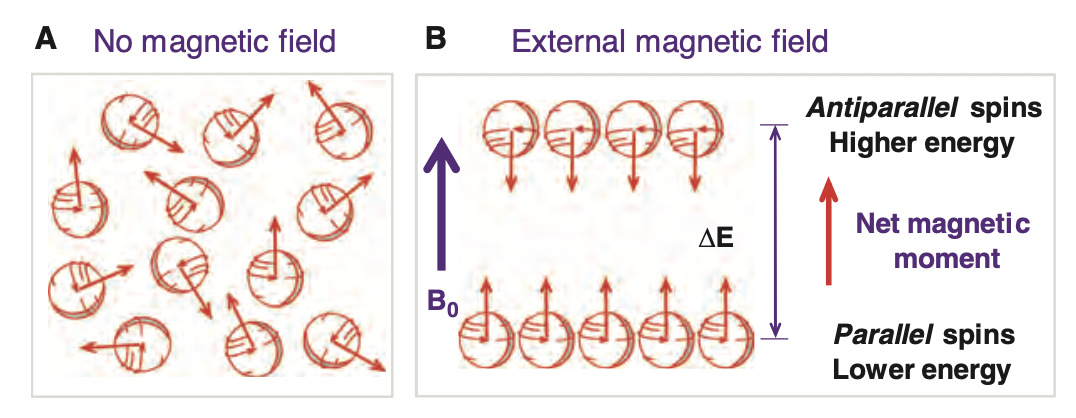
\includegraphics[width=\textwidth]{Assets/MRIproton.png}
	\caption[Proton alignment in a magnetic field]{Schematic illustration of how hydrogen protons ($^1$H) behave in the presence of a strong static magnetic field ($B_0$). 
		A: In the absence of a field, proton magnetic moments are randomly oriented, producing no net magnetization. 
		B: When exposed to $B_0$, protons align either parallel or antiparallel to the field. 
		From Bushberg, J.T., \textit{The Essential Physics of Medical Imaging} (2011) \cite{bushberg2011}.}
	\label{fig:proton_alignment}
\end{figure}


Depicted in Figure \ref{fig:protonPrecession}, the motion happens around the axis of the applied magnetic field due to the perpendicular torque they experience. 

\begin{figure}[htb!]
	\centering
	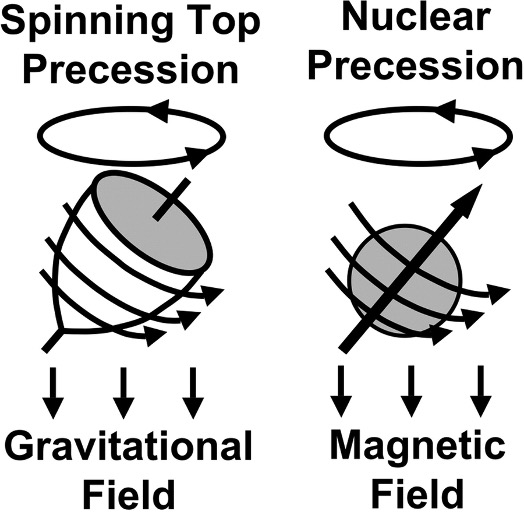
\includegraphics[width=0.55\linewidth]{Assets/protonPrecession.jpg}
	\caption[Analogy between proton spin precession and precession of a spinning top.]{Illustration of proton precession under a static magnetic field $B_0$ compared to that of a spinning top under gravity. Adapted from Pooley, R. A., \textit{Fundamental physics of MR imaging}, (2005) \cite{Pooley2005}.}
	\label{fig:protonPrecession}
\end{figure}

%Precession and Larmor frequency
In addition to aligning with $B_0$, the protons also experience precession, much like the Earth’s rotation around its tilted axis or a spinning top under gravity. This precession occurs at an angular frequency ($\omega_0$) known as the Larmor frequency, which is directly proportional to the magnetic field strength ($B_0$), as described by the Larmor equation $\omega_0 = \gamma B_0.$

%RF coils role
An \gls{rf} energy pulse ($B_1$) is then applied, synchronized to the Larmor frequency of protons (about 42.58 MHz per tesla), magnetizing the protons and tipping the net magnetization ($M$) away from the longitudinal direction ($M_z$). This pulse provides just enough energy for some protons to move into a higher energy state, also called RF excitation. In doing so, it also causes the magnetic moments of many protons to become synchronized, or phase-coherent. They start to precess together in the transverse plane, creating what is called transverse magnetization ($M_{xy}$).

The instant the RF pulse is turned off, the relaxation process starts, these precessing protons start to lose that synchronization due to slight variations in their local magnetic environments. This causes the transverse magnetization signal to gradually fade over time. The oscillations of this signal are detected by the same RF coils that sent them. %The strength and rate of decay of this signal are dependent on the tissue type and are characterized by two time constants: $T1$ and $T2$.

First, the signal in the transverse plane, ($M_{xy}$), decreases as the protons desynchronize, this is described by $T2$ (Transverse Relaxation). And the process by which the system regains equilibrium is described by $T1$ (Longitudinal Relaxation).  The longitudinal magnetization ($M_z$) returns, and the particles realign with the main magnetic field ($B_0$). The final \gls{mri} image's depiction of a tissue's brightness or darkness is determined by the RF signal produced during relaxation processes taken together.  %For instance, on $T1$-weighted images, tissues with short $T1$ times (such as fat) seem bright, whereas on $T2$-weighted images, tissues with longer $T2$ periods (such as cerebrospinal fluid) appear bright, see Figure~\ref{fig:T2vsT1}.

%\begin{figure}[htb!]
	%\centering
	%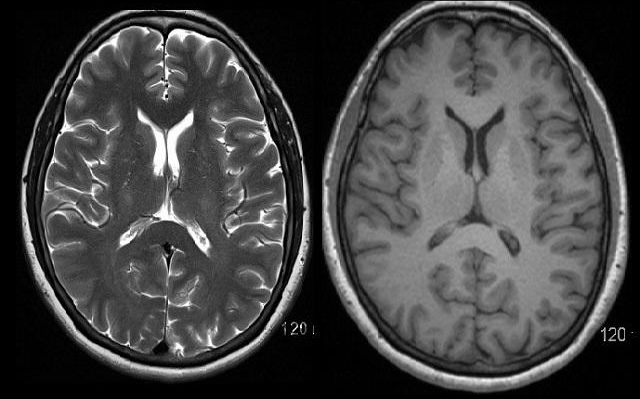
\includegraphics[width=0.65\textwidth]{Assets/T2vsT1.jpg}
	%\caption[Comparison between T1- and T2-weighted brain MRI images.]{Comparison between T1- and T2-weighted brain MRI images of the same subject. The left image shows a T2-weighted scan, where cerebrospinal fluid (CSF) appears bright, and the right image shows a T1-weighted scan, where fat and white matter appear bright. Adapted from \cite{riteadvantageT1T2}.}
	%\label{fig:T2vsT1}
%\end{figure}

%gradient fields role
However, this covers one a single signal from a particular spot. To make an image rather, the \gls{mri} system must know where each signal is coming from. This is achieved using small, precisely controlled variations in the magnetic field known as gradient fields. These gradient coils, superimposed on $B_0$, make the magnetic field slightly stronger or weaker depending on position, causing the Larmor frequency of the protons to vary with location.

Three gradient systems work together to map space. First, \gls{ssg} is a applied during excitation so that only protons in a particular “slice” of the body resonate at the RF pulse frequency. This defines the plane of imaging. Then, \gls{peg}, briefly changes the precession speed of protons in one direction, giving each row of tissue a unique phase ``signature". Finally, \gls{feg} is applied during signal readout so that protons along another axis precess at slightly different frequencies.

%\subsection{Scanner Design and Subsystems}

%As mentioned above, after the main static field ($B_0$) has been established and shimmed to high homogeneity the gradient coils introduce controlled spatial variation in the magnetic field for encoding localizing signals generated during MR. Gradient coils, are wire conductors located within the main bore of the magnet with typical strength values from 1 to 50 mT/m and correspond to the logical coordinate axes: x, y, and z which relate to \gls{ssg}, \gls{peg}, and \gls{feg}. They operate by adding to or subtracting from the magnitude of the main field ($B_0$), but they do not change the direction of the magnetic field \cite{bushberg2011}.

These gradients must switch rapidly and with large current flows, typical slew rate ranges from 5 to 250 mT/m/ms, with currents on the order of 100–200 A \cite{bushberg2011,Prince_MedicalImaging_2015}, to accomplish encoding. The resulting signals are stored in a matrix called k-space. Each line in k-space represents one measurement with a specific gradient configuration. When all necessary lines are filled, the Fourier Transform reconstructs the data into an image, where each pixel corresponds to a small volume element (voxel) of tissue.

The control and computing subsystems coordinate every stage of image acquisition and reconstruction. The host computer and operator console provide the interface through which the technologist selects and supervises scanning protocols, while the pulse programming and measurement control systems synchronize gradient and RF activity \cite{bushberg2011}. Supporting units such as the digitizer, image processor, and compute engine translate the raw analog signals into interpretable digital images through Fourier-based reconstruction algorithms \cite{Prince_MedicalImaging_2015}; Finally, the dedicated power supplies, patient table mechanics, and electromagnetic shielding ensure stable operation, patient positioning, and noise minimization. 

These same magnetic field components pose hazards can pose hazards to implanted conductive objects. Although most modern \gls{mri} systems are designed for patient safety, implanted devices and retained surgical materials introduce additional considerations. One clinically relevant example is epicardial leads, which are commonly placed during cardiac surgery to provide temporary postoperative pacing for arrhythmias. These leads consist of conductive wires (often stainless steel or similar alloys) sutured directly to the epicardial surface of the heart and may be removed postoperatively or, in some cases, cut short and abandoned in situ to avoid extraction risks.